% ----------------------- Vorlage einlesen ---------------------------
% Dokumentenklasse festlegen
\documentclass[a4paper, 12pt, chapterprefix=false]{scrreprt}

% ----------------------- Packages importieren ---------------------------

\usepackage[utf8]{inputenc}
\usepackage[ngerman]{babel}
\usepackage{amsmath}
\usepackage{amssymb}
\usepackage{fancyhdr}
\usepackage{color}
\usepackage{graphicx}
\usepackage{lastpage}
\usepackage{pdflscape}
\usepackage{subfigure}
\usepackage{float}
\usepackage{polynom}
\usepackage{forloop}
\usepackage[a4paper]{geometry}
\usepackage{listings}
\usepackage{fancybox}
\usepackage{tikz}
\usepackage{algpseudocode,algorithm,algorithmicx}
\usepackage[onehalfspacing]{setspace}
\usepackage{booktabs}
\usepackage{multirow}
\usepackage{tabularx}
\usepackage{hyperref}
\usepackage{blindtext}
\usepackage{pdfpages}
\usepackage{enumitem}
\usepackage{parskip}




% ----------------------- Seitenlayout ---------------------------

% Größe der Ränder setzen
\geometry{a4paper, left=2.5cm, right=2.5cm, top=2.5cm, bottom=2.5cm}
\parindent= 0pt

% Kopfzeile 
\pagestyle {fancy}
\fancyhead[L]{\Modul}
\fancyhead[C]{Team Gyrocopter}
\fancyhead[R]{\today}

% Fußzeile
\fancyfoot[L]{}
\fancyfoot[C]{}
\fancyfoot[R]{Seite \thepage /\pageref*{LastPage}}


% ----------------------- Layout Überschriften / Abschnitte ---------------------------

\renewcommand*\chapterheadstartvskip{\vspace*{-\topskip}}
\renewcommand*\chapterheadendvskip{
\vspace*{1\baselineskip plus .1\baselineskip minus .167\baselineskip}}



\setkomafont{chapter}{\fontsize{17bp}{18.8bp}\selectfont\bfseries}
\setkomafont{section}{\fontsize{15bp}{18.8bp}\selectfont\bfseries}
\setkomafont{subsection}{\fontsize{13bp}{18.8bp}\selectfont\bfseries}


% Abstand Auflistung ändern
\setitemize{itemsep= -2pt}
\setenumerate{itemsep= -2pt}
\setstretch{1.15}
\setlength{\parskip}{1pt}
% ----------------------- Erstellung neuer Kommandos ---------------------------
\newcommand{\Heading}{Team Gyrocopter}
\newcommand{\Modul}{Projekt Data Science}

\newcommand{\Dozent}{Dozent: Prof. Dr. Christian Hänig}


% ----------------------- Beginn Dokument ---------------------------
\begin{document}
% ----------------------- Vorlage Titelseite einlesen ---------------------------
\begin{titlepage}


\begin{figure}[h]
\begin{center}

\includegraphics[width=10cm]{../../data/HSA_Logo}
\end{center}\label{fig:hsa_logo_figure}
\end{figure}

\begin{center}

\vspace{3.5 cm}


{\Huge \textbf{\Heading}}

\vspace{1.3 cm}

{\Huge \textbf{Modul: \Modul}}\\

\vspace{3 cm}

\begin{onehalfspace}


\begin{large}

\Semester \\


\Dozent \\


\vfill




Gruppe: Timo van den Wyenbergh und Felix Graß\\

Studiengang Data Science M.Sc.\\

Sommersemester 2022\\


\end{large}
\end{onehalfspace}

\end{center}


\end{titlepage}

\newpage % ----------------------- Neue Seite ---------------------------


\tableofcontents % Inhaltsverzeichnis

\thispagestyle{empty}

\newpage % ----------------------- Neue Seite ---------------------------
\setcounter{page}{1} % Blattnummerierung

\chapter{Konzept}\thispagestyle{fancy}

\section{Kontext}

Bei der Findung eines geeigneten Themas für die Projektarbeit des Modul \glqq Projekt Data Science\grqq{}  suchten wir
nach einer Problemstellung im Bereich der Bildverarbeitung von Luftaufnahmen.
In diesem Zusammenhang lernten wir Herrn Prof. Dr. Bannehr vom Fachbereich 3 der Hochschule Anhalt kennen.
Herr Bannehr befasst sich mit dem Aufgabengebiet der Geodatenerfassung und besitzt am Fachbereich unter anderem einen
Gyrocopter, mit dem er bereits mehrere Befliegungen durchführte.
Für unsere Projektarbeit erhielten wir von Herrn Bannehr die Luftaufnahmen von Oldenburg und Dessau und überlegten uns
nach Begutachtung der Datengrundlage eine geeignete Aufgabenstellung.

\section{Datengrundlage}
Die Datengrundlage umfasste die Luftaufnahmen der Befliegung von Oldenburg und Dessau.
Dabei handelte es sich bei den Datenformaten um Hyperspektral-, Thermal- und Höhenmeter-Daten.
Leider wurde bei der Befliegung von Dessau aber keine Thermaldaten aufgenommen und weil das übermittelte Gesamtbild
Prozessierungsfehler erhielt verwendeten wir nur die Daten von Oldenburg.

\section{Aufgabenstellung}
Bei der anfänglichen Aufgabenstellung von Herrn Bannehr handelte es sich um einen Klassifikationsvergleich von Dachmaterialien.
Geplant war der Vergleich der Ergebnisse der Methoden des Fachbereichs 3 zu unseren Ergebnissen mit mehr individualisierbaren Methoden.
Da sich nach den ersten Wochen der Bearbeitung herausstellte, dass es keine annotierten Daten gibt und keine Vergleichsarbeit existiert,
änderten wir unter Absprach mit Herrn Bannehr das Thema.\\
Die neue Aufgabenstellung befasste sich nun mit der Bildsegmentierung der Luftaufnahme in acht Klassen, die fast vollständig
das Bild beschreiben. Zu den klassifizieren Instanzen gehören Wiese, Wald, Schienen, Straße, Auto, See, Häuser und None.

\section{Projektbestandteile und Zeitplan}
Für die Projektplanung setzten wir uns für jeden Schritt im Cross Industry Standard Process for Data Mining eine Deadline
und bildeten dementsprechend unsere Work-Packages.

\begin{center}
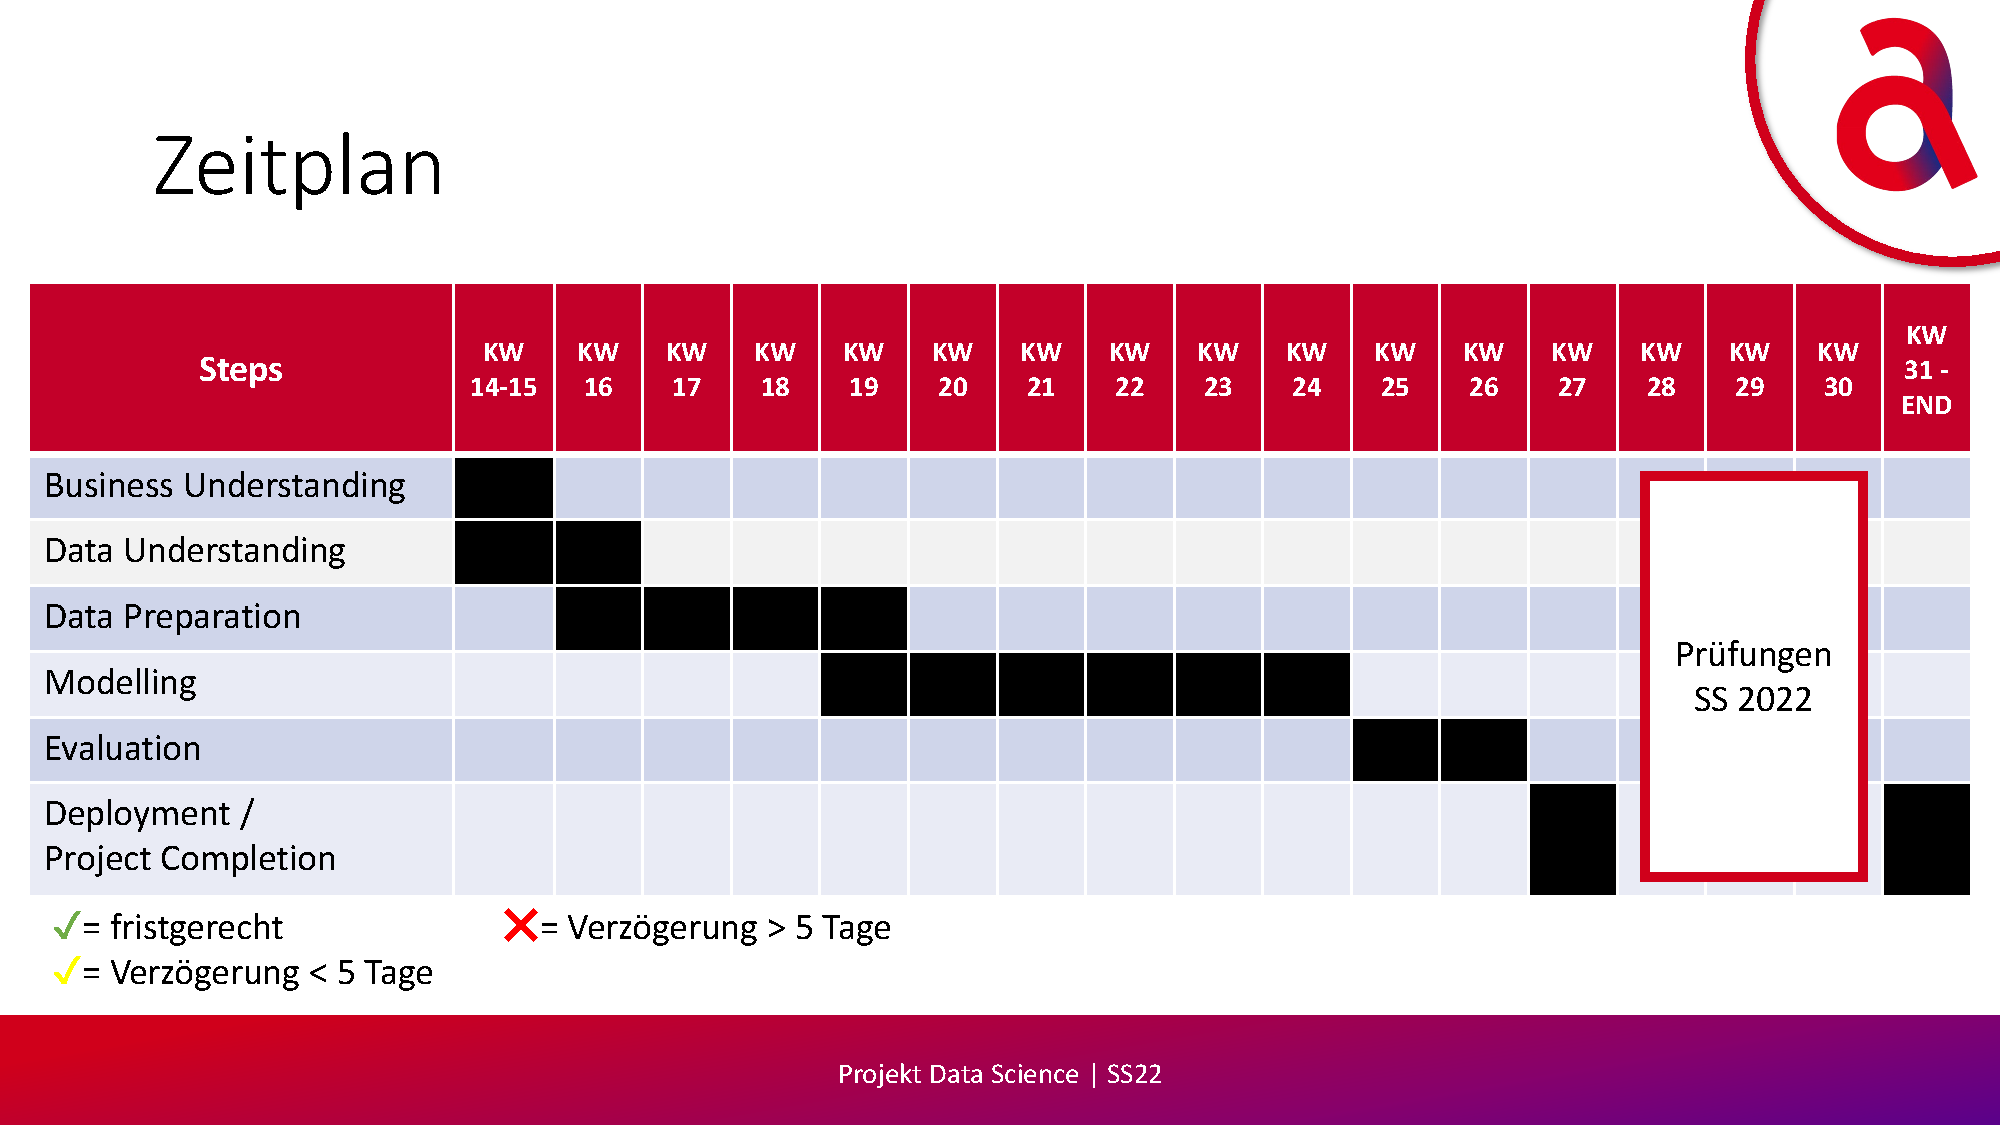
\includegraphics[width=15cm]{../../data/Zeitplan}
\end{center}

\subsection{Bussines und Data Unterstanding}
Zu Beginn des Projektes mussten wir uns in die Thematik einarbeiten und eine geeignete Aufgabenstellung finden.
Wir führten eine Recherche zum Thema \glqq Analyse von Hyperspektraldaten mit Hilfe von Python\grqq{}  durch und arbeiteten an
dem Import der zur Verfügung gestellten Daten.

\subsection{Data Preparation}
Der Großteil des Projekts beschäftigte sich mit der Datenaufbereitung bzw. -vorverarbeitung.
Von Beginn an war klar, dass das Gesamtbild mit 3500x1980 Pixel nicht als Ganzes verarbeitet werden kann und wir Teilbilder erzeugen müssen.
Des Weiteren mussten Bilder annotiert werden und dessen Label den Bildern zugeordnet werden.
Somit wurde im Teil Data Preparation mehrere Funktionen erstellt, die die im Folgenden aufgelisteten Aufgaben erledigen.

\begin{itemize}
    \item Hyperspectral-, Thermal- und Oberflächendaten zusammenführen
    \item Ein Gesamtbild in mehrere Teilbilder zerlegen
    \item Mehrere Teilbilder zu einem Gesamtbild zusammenführen
    \item RGB- und DOM-Bilder von Teilbildern erzeugen
    \item Umwandlung der Annotation vom XML-Format in ein Label-Band
\end{itemize}

Der Aufwand der Annotation sollte man hierbei jedoch nicht unterschätzen.

\subsection{Modelling}
Im Bereich des Modellings wendeten wir neben den bekannten Modellen wie z.B. K-Nearest-Neighbors und
einfachen Neuronalen Netzen, gängige Convolutional Neural Networks (CNN) zur Bildsegmentierung an.
Vor der eigentlichen Modellierung mussten wir uns zu Beginn in die Programmierbibliotheken und Model-Monitoring-Tools
einarbeiten.

\subsection{Evaluation}
Anschließend an das Modelling verglichen wir fortlaufend welche Modelle besser performen und welche Ursachen für
schlechte Modellergebnisse verantwortlich sein könnten.
In diesem Kontext führten wir auch ein Inter-Annotator-Agreement durch und verbesserten unsere Annotationsrichtlinien.

\subsection{Deployment / Project Completion}
Zum Projektende galt es die Gesamtarbeit final zu ordnen und für Dritte verständlich zu vervollständigen.
Dabei erstellten wir ein Script, dass die Modellvorhersagen für das Gesamtbild durchführt und mit den selbst
definierten Farbwerten als RGB-Bild abspeichert.
Zuletzt vervollständigten wir noch Lücken in der Quelltext-Dokumentation und kontrollierten die erforderlichen
Anforderungen für die Abgabe.


\newpage % ----------------------- Neue Seite ---------------------------

\chapter{Projektzusammenfassung}\thispagestyle{fancy}

\section{Aufgabenstellung}
Im Rahmen dieses Projektes sollen Luftaufnahmen in bis zu 8 Klassen segmentiert werden.
Zu den klassifizieren Instanzen gehören Wiese, Wald, Schienen, Straße, Auto, See, Häuser und None.
Die verwendeten Luftaufnahmen stammen aus Befliegung der Stadt Oldenburg aufgenommen vom Gyrocopter des Fachbereichs 3
der Hochschule Anhalt.
Die Daten umfassen Hyperspektral-, Thermal- und Höhenmeter-Daten.

\section{Verwendete Tools}
Die gesamte Entwicklung wurde in Python umgesetzt.
Hierzu wurde insbesondere das Paket spectral zur einfachen Verarbeitung von envi-Daten verwendet.

\section{Datenvorverarbeitung}
Die Aufnahmen wurden jeweils als getrennte Dateien für Hyperspektral-, Thermal- und Höhenmeterdaten zur Verfügung gestellt.
Im ersten Vorverarbeitungsschritt wurden diese zusammengeführt, indem die Thermal- und Höhenmeterdaten als einzelne Bänder an die Hyperspektraldaten angefügt wurden.
Hierbei war von Vorteil, dass die verschiedenen Daten das exakt gleiche Gebiet umfassten, sodass eine Georefferenzierung von Koordinatenpunkten nicht notwendig war.
Für die weiteren Verarbeitungsschritte musste das Luftbild in viele Teilbilder unterteilt werden.
Als Größe haben wir uns für 200x200 Pixel entschieden, da hierdurch bei geringem Informationsverlust der notwendige Rechenaufwand der Neuronalen Netze erheblich reduziert wird.


\section{Annotation}
Da keine annotierten Bilder zur Verfügung standen musste ein Teil der Bilder annotiert werden.
Hierfür wurde aus verschiedenen Anwendungen das Online Tool Roboflow aufgrund seiner hervorragenden Nutzoberfläche ausgewählt.
Trotz mehrfacher Anpassung unserer Annotationsrichtlinien konnten wir die RGB Teilbilder nicht konsistent genug annotieren.
Insbesondere die Unterscheidung von Bäumen und Sträuchern (klassifiziert als Wiesen) war auf dieser Basis nicht möglich.
Unter gleichzeitiger Betrachtung der Höhendaten war eine Annotation mit einer Übereinstimmung von ca.75\% möglich.

\section{Augmentation}

\section{Modellierung}

\subsection{Baseline}
Als Baseline diente ein einfacher Pixel-basierter Ansatz. Hierbei ist jede Instanz ein Pixel und enthält ausschließlich
die Hyperspektral-, Thermal- und Höhenmeter-Daten dieses Pixels.
Modelliert wurde die Baseline durch ein Neuronales Netz(NN) mit folgender Struktur:

\begin{figure}[h]
\begin{center}
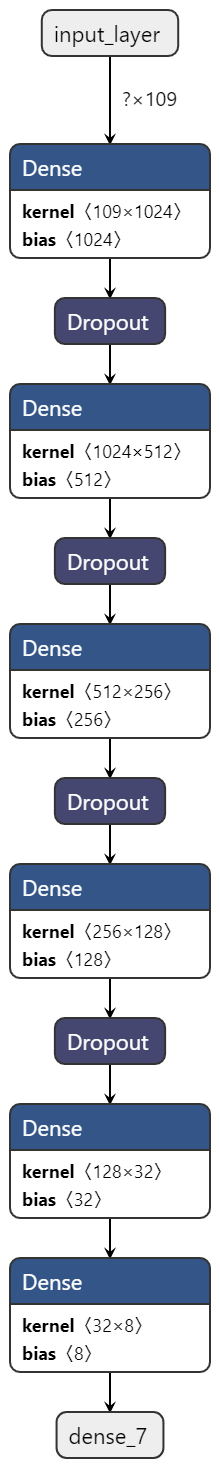
\includegraphics[angle=90, width=15cm]{../../data/models/baseline3_nn_for_pixel}
\end{center}
\end{figure}

\subsection{CNN}

\section{Evaluierung}


\section{Hyperparametertuning}

\section{Verbesserungspotenzial}

\section{Learnings}


\end{document}
